% Festlegen des Dokumententyps
\documentclass[a4paper,twoside]{scrartcl}
\addtokomafont{caption}{\footnotesize}

% Papierformat
\usepackage{a4}

% Deutsche Sprache (Silbentrennung, usw.)
\usepackage[ngerman]{babel}
\usepackage[babel,german=quotes]{csquotes}

% Schrifteneinstellungen
\usepackage{lmodern}
\usepackage[T1]{fontenc}
\usepackage{textcomp}

% Kodierung
%\usepackage{ucs}
\usepackage[utf8]{inputenc}

% bessere Matheunterstützung
\usepackage{amsfonts}
\usepackage{amstext}
\usepackage{amsmath}

% Einheiten in Formalen0
\usepackage{siunitx}
\sisetup{%
locale=DE,
scientific-notation = true,
}

% fuer Zitate
\usepackage[natbib=true,style=numeric]{biblatex}
\bibliography{literature}

% Grafiken einbinden
\usepackage{graphicx}

% Grafiken Position erzwingen
\usepackage{here}

% Tabellen
\usepackage{booktabs}

% Verweise in PDF-Dateien
\usepackage
[colorlinks,
pdfstartview = 1,
bookmarksopen = true,
bookmarksnumbered = true,
linkcolor = black,
plainpages = true,
hypertexnames = false,
citecolor = black]{hyperref} 

% PGF einbinden
\usepackage{tikz}
\pgfrealjobname{protocol}
\newcommand{\inputTikZ}[1]{%
    \resizebox{\textwidth}{!}{\input{#1.pgf}}%
  }

\newcommand{\e}{{\rm e}}

\begin{document}

\thispagestyle{empty}
\begin{center}
    {\Huge{\textbf{Physikalisches Praktikum}}}\\[16pt]
\ \\
\ \\
\ \\
\ \\
\ \\
\ \\
\ \\
\ \\
\ \\
\ \\
\ \\
\ \\
\ \\
\ \\
\ \\
\ \\
\ \\
\huge{Die Potenzialwaage}
\ \\
\ \\
\large{Versuch 10}
\end{center}

\normalsize
\ \\
\ \\
\ \\
\ \\
\ \\

\begin{center}
\begin{tabular}{lcl}
      Name: & ~ & Daniel Elkeles \\
                    & ~ & E-Mail: daniel.elkeles@stud.uni-goettingen.de \\
	  		& ~ & Tom Groß \\
		    		& ~ & E-Mail: tom.gross@stud.uni-goettingen.de \\
\ \\		    
      Tutorin: & ~ & Jantje Freudenthal \\
      Gruppe: & ~ & 10 \\
\ \\      
      Durchgeführt am: & ~ & 03.06.2013 \\
      Protokoll abgegeben: & ~ & 17.06.2013 \\
      Protokoll verbessert: & ~ & ........................\\
\ \\
\ \\
      Testiert: .................................    
\end{tabular}\\
\end{center}

\newpage
%Seitennummerierung ausschalten
\thispagestyle{empty}
\tableofcontents
\newpage
%Seitenzähler zurücksetzen
\setcounter{page}{1}
\section{Einleitung}

%\newpage
\section{Theorie}
\subsection{Elektronenstrahl}
Ein Elektronenstrahl wird i.A., so auch bei diesem Experiment, mithilfe einer Glühkathode in Kombination mit einem Wehneltzylinder
erzeugt.
Zuerst eine sogenannte Heizspule mit der Heizspannung $U_H$ zum Glühen gebracht. Die dadurch freigesetzten Elektronen werden in einer
Zylinderkathode (Wehneltzylinder) auf den Mittelpunkt dieser fokussiert und dann durch eine Anodenplatte mit einem kleinen Loch in 
der Mitte beschleunigt.\\
%\begin{center}
\begin{minipage}{5cm}
\centering
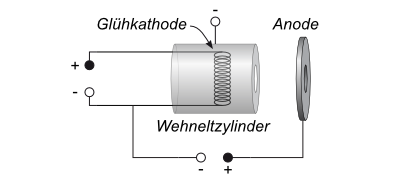
\includegraphics{Elektronenkanone.png}
\end{minipage}\\
%\end{center}

\subsection{Helmholtzspule}
Die Helmholtzspule ist eine Apparatur zur Erzeugung eines homogenen Magnetfeldes. Das wird erreicht, indem zwei Leiterschleifen vom 
Radius $R$ parallel zueinander von einem Strom durchflossen werden. Für das Magnetfeld ergibt sich durch Symmetrie nur eine Abhängigkeit
von der $\hat{e}_z$-Achse, sodass sich das Magnetfeld ergibt zu:
\begin{align}
B_{z} & = \frac{1}{2} \mu_{0} \mu_{r} n I R^2 \left[ \left( R^2+ \left( z - \frac{R}{2} \right)^2 \right)^{- \frac{3}{2}} + \left( R^2 + \left( z + \frac{R}{2} \right)^2 \right)^{- \frac{3}{2}} \right] \text{.} 
\end{align}

\subsection{Herleitung $\frac{e}{m_e}$}
Zur Herleitung des Quotienten $\frac{e}{m_e}$ kann man das Kräftegleichgewicht betrachten. Dazu werden folgende zwei Kräfte betrachtet:
\begin{itemize}
\item Lorentzkraft $\vec{F}_L$
\item Zentripetalkraft $\vec{F}_Z$
\end{itemize}
Die Lorentzkraft ist die Kraft, die auf ein Elektron in einem $\vec{E}$- oder $\vec{B}$-Feld wirkt:
\begin{align*}
\vec{F}_L&=q\left(\vec{E}+\vec{v}\times\vec{B}\right)\text{.}
\end{align*}
Da wir bei unserem Experiment nur ein Magnetfeld betrachten, also $\vec{E}=0$, lässt sich die Lorentzkraft auch schreiben als:
\begin{align}
\vec{F}_L&=q\vec{v}\times\vec{B}.
\end{align}
Die Zentripetalkraft $F_Z$ hingegen ist die Kraft, die auf ein um einen festen Punkt rotierenden Körper wirkt:
\begin{align}
\vec{F}_Z&=\frac{m_ev^2}{r}\text{.}
\end{align}
In unserem Fall sind beide Kräfte gleich, wenn das Elektron im $\vec{B}$-Feld im Kreis rotiert. In diesem Fall lässt sich der für
unser Experiment gesuchter Radius $r$ bestimmen.

\begin{align}
F_Z&=F_L \\
\frac{m_ev^2}{r}&=q\vec{v} \times \vec{B} \\
\Rightarrow \frac{e}{m_e}&=\frac{v}{Br}
\end{align}
Durch Einsetzen des Magnetfeldes ergibt sich für den Quotienten $\frac{e}{m_e}$:
\begin{align}
\frac{e}{m_e}&=\frac{125U_BR^2}{32\left(r\mu_0\mu_rnI\right)^2}\text{.}
\end{align}
%\newpage
\section{Durchführung}

%\newpage
\section{Auswertung}

%\newpage
\section{Diskussion}

\newpage
\thispagestyle{empty}
% Festlegung Art der Zitierung - Havardmethode: Abkuerzung Autor + Jahr
\printbibliography
\appendix
\section{Messwerte (Original)}
\end{document}